%%=============================================================================
%% Methodologie
%%=============================================================================

\chapter{\IfLanguageName{dutch}{Methodologie}{Methodology}}
\label{ch:methodologie}

\section{Inleiding}
Om een antwoord te krijgen op de onderzoeksvraag wordt een experiment opgesteld. In dit experiment wordt een mobiele applicatie ontwikkeld voor de, reeds opgesomde, benaderingen van State Management. Dit experiment zal, per benadering van de verschillende State Management, twee resultaten opleveren. Het eerste resultaat zal het aantal lijnen code van het project bevatten per benadering. Hoe deze meting te werk zal gaan wordt in sectie \ref{ch:loc} besproken. Als tweede resultaat wordt een automatische procedure een aantal keer doorlopen, dit wordt uitvoerig besproken in sectie \ref{ch:prestaties}. \newline
Als eerst worden de nodige voorbereidingen voor dit experiment besproken.

\section{Voorbereidingen}
\subsection{De applicatie}
De applicatie heet ``Store It'. Het hoofddoel van de applicatie is om producten te bekijken en toe te voegen. De koper heeft als doel de lijst van producten te raadplegen. Alsook de details van een product te bekijken en eventueel een product te verwijderen. Een verkoper heeft als hoofddoel om een product toe te voegen. Om de complexiteit van de applicatie te beperken wordt geen onderscheid gemaakt tussen een klant en een verkoper.\newline

De layout van de mobiele applicatie is gebasseerd op mock-ups, zie figuren \ref{fig:mock-ups-store-it}. Deze mock-ups werden op voorhand gemaakt zodat tijdens het ontwikkelen van de applicatie geen tijd besteed wordt aan de visuele aspecten.

\begin{figure}
    \begin{tabular}{cc}
        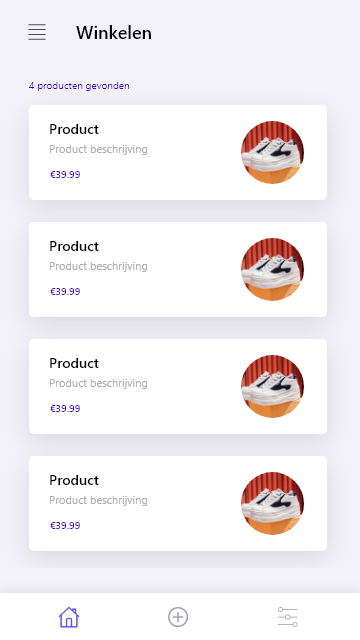
\includegraphics[width=65mm]{img/methodologie/mock-home_screen.png} &   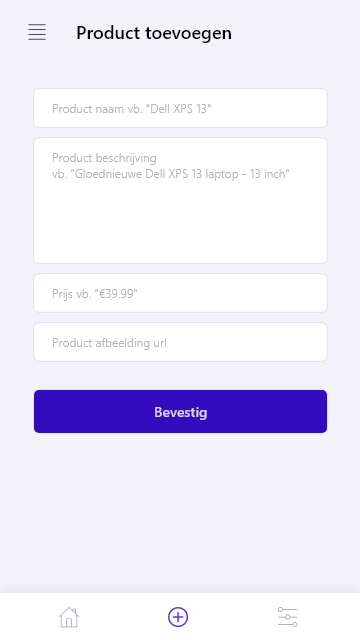
\includegraphics[width=65mm]{img/methodologie/mock-add_product_screen.png} \\
        (a) Mock-up: product lijst pagina & (b) Mock-up: product toevoegen pagina\\[6pt]
        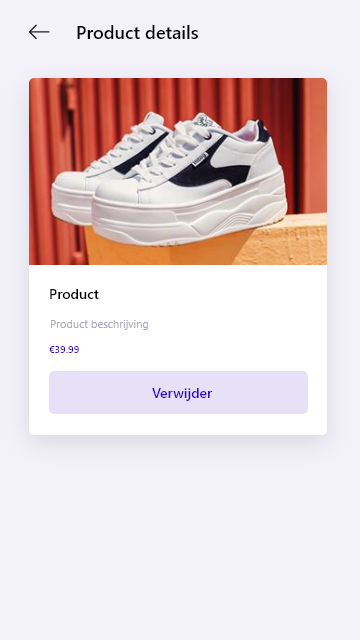
\includegraphics[width=65mm]{img/methodologie/mock-details_screen.png} &   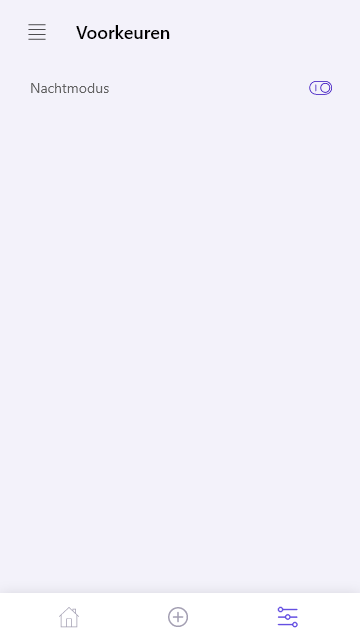
\includegraphics[width=65mm]{img/methodologie/mock-preferences.png} \\
        (c) Mock-up: product details pagina & (d) Mock-up: Voorkeuren pagina \\[6pt]
    \end{tabular}
    \caption{Mock-ups van Store It}
    \label{fig:mock-ups-store-it}
\end{figure}

\subsection*{Schermen}
De Store It applicatie bestaat uit vier schermen: 
\begin{itemize}
    \item De ``start'' pagina met een lijst van de producten
    \item De ``voeg-product-toe'' pagina met een formulier om een product toe te voegen
    \item De ``voorkeuren'' pagina met een mogelijkheid om het thema van de applicatie te wijzigen
    \item De ``details'' pagina met de details van een geselecteerd product
\end{itemize}

De Store It applicatie maakt het navigeren mogelijk met een \verb|BottomNavigationBar|. De applicatie start op de startpagina, waar de lijst met beschikbare producten wordt weergegeven. Om de geselecteerde tab van de bottom navigation bar bij te houden, wordt gebruikt gemaakt van een index. Deze index wijzigt wanneer een gebruiker op een item in de bottom navigation bar klikt. Om de state bij te werken voor het wijzigen van de index wordt gebruik gemaakt van \verb|setState()|. De index van de startpagina, voeg-product-toe pagina en voorkeuren pagina zijn respectievelijk 0, 1, 2.
Op basis van deze index wordt de bijhorende pagina getoond.

Wanneer een gebruiker op een product klikt, wordt de detailspagina geopend. \newline
De gebruiker heeft de mogelijkheid om het product te verwijderen op de detailspagina. Indien het product is verwijderd, wordt een snackbar getoond met een bevestiging en wordt de gebruik herleid naar de startpagina.
De detailspagina is de enige pagina die bovenop de actieve pagina wordt gepusht. Deze pagina beschikt over een terug knop die de detailspagina zal ``poppen''.

Op de voeg-product-toe pagina wordt een invulformulier getoond. Hier kan de gebruiker een nieuw product toevoegen. De invoervelden beschikken over standaard validatie waarbij de ingevoerde waarde niet leeg mag zijn. Indien deze validatie niet is voldaan, wordt een gepaste melding onder desbetreffend invoerveld getoond. \newline
Wanneer de gebruiker bevestigt, wordt het product toegevoegd aan de lijst op de startpagina. Merk op dat op dit moment deze productlijst niet getoond wordt aangezien de gebruiker zich op de voeg-product-toe pagina bevindt.

Op de voorkeurenpagina kan de gebruiker het thema aanpassen, dit gebeurt met de \verb|Switch| widget. Standaard start de applicatie in een licht thema. De gebruiker kan naarmate zijn/haar voorkeuren het thema aanpassen. De mogelijke thema's zijn licht en donker.
Wanneer het thema wijzigt, wordt de gehele applicatie aangepast naar het geselecteerde thema. Aangezien de gehele applicatie moet gewijzigd worden, is dit een interessante pagina op vlak van state. Namelijk elk widget in de widget tree moet opnieuw gebouwd worden om de wijzigingen ``at runtime'' toe te passen.


De broncode is beschikbaar op \url{https://github.com/devrnt/bachelor-thesis-store-it}\autocite{Vrient2019}. De \verb|master| tak bevat de boilerplate code. De verschillende benaderingen zijn onderveeld per tak. Zo bevat de \verb|mobx| tak de MobX State Management benadering.

\section{Aantal lijnen code}
\label{ch:loc}
Om een benaderend meetniveau te verkrijgen voor de complexiteit van een State Management worden de aantal lijnen code geteld. Dit resultaat zal een beeld scheppen op de hoeveelheid code die geschreven moet worden om een benadering van State Management uit te schrijven. Merk op dat de complexiteit van een benadering verschillend is van ontwikkelaar tot ontwikkelaar, dit is en blijft een subjectief meetniveau. Uit dit resultaat wordt besloten hoe vlot een benadering van State Management geschreven kan worden. Dit kan leiden tot bijvoorbeeld volgende conclusie: Flutter beginners zullen de voorkeur geven aan benaderingen die vlugger zijn uit te schrijven. 

De aantal lijnen code van de Dart bestanden worden geteld. De Dart bestanden worden gekenmerkt door de \verb|.dart| extensie. Hiervoor wordt per verschillende benadering het volgende commando gebruikt: \verb=find . -name '*.dart' \| xargs wc -l=. Dit commando geeft het totaal aantal lijnen code terug, dit zal per verschillende benadering uitgevoerd worden. \newline 
Tijdens het schrijven van de benaderingen wordt er rekening gehouden met volgende afspraken: commentaar in de code wordt, voor het commando wordt uitgevoerd, verwijderd. Er wordt enkel gebruik gemaakt van een backspace (nieuwe lijn) voor de scheiding van de verschillende methodes. Deze afspraken worden strict nagestreefd doorheen de verschillende benaderingen. \newline
\newline
Vooraleer de aantal lijnen code worden geteld, wordt de broncode van de verschillende benaderingen geformateerd. In dit experiment wordt de \verb|dart_style| package gebruikt als formatter. Deze formatter hanteert de richtlijnen van de Dart style guide \autocite{Dart2019a}. De \verb|line-length| wordt ingesteld op negentig. Dit houdt in, dat lijnen die langer zijn dan 90 karakters, gebroken worden en op een nieuwe lijn verder lopen.


\section{Prestaties}
\label{ch:prestaties}
\subsection{Integratietesten}
Flutter beschikt over de nodige tools voor het uitvoeren van integratie testen. Deze testen schrijven de gebruikersflow uit, waardoor individuele modules als één geheel getest kunnen worden. Tijdens een integratie test wordt een gebruikersflow uitgeschreven en vervolgens gesimuleerd op een apparaat \autocite{Flutter2019b}. \newline 

Een integratie test bestaat uit de eindapplicatie, die ook gebruikt zou worden in productie, en een test suite. De test suite definieert de stappen die doorlopen worden tijdens de integratie test. Een voorbeeld van een flow: \textit{De gebruiker klikt op een product, vervolgens verwijdert de gebruiker het product...}. Zie \ref{ch:user-flow} gebruiker-flow voor dit experiment. De test suite vindt de nodige widgets in de applicatie door een unieke \verb|key| te definiëren in de broncode. In de test suite wordt het widget opgeroepen met: \verb|find.byValueKey('product-item')|. \newline
Deze integratie testen worden in dit experiment gebruikt om de automatische gebruiker-flow uit te schrijven. Zodanig dat telkens hetzelfde pad wordt doorlopen per benadering van State Management.

Om de effectieve integratie testen te schrijven wordt de \verb|flutter_driver| package gebruikt.
Een integratie test maakt een instrumentale versie van de applicatie. Deze instrumentale versie maakt het mogelijk om de applicatie te besturen (met de stappen uit de test suite) en prestaties te capteren.
De integratie testen worden uitgevoerd in de profile modus van Flutter. De profile modus compileert en start een applicatie bijna identiek als de release mode (productie) en beschikt over de extra functionaliteit om prestatieproblemen te capteren en te debuggen.

\subsection{Gebruikersflow}
\label{ch:user-flow}
In dit experiment ligt de focus van de verschillende benaderingen van State Management op volgende zaken: 
\begin{itemize}
    \item De gebruiker wijzigt het thema op de voorkeurenpagina.
    \item De gebruiker voegt een nieuw product toe, als gevolg dat de lijst van producten moet bijgewerkt worden op de andere pagina.
    \item De gebruiker verwijdert een product op het detailspagina, als gevolg dat de lijst van producten moet bijgewerkt worden op de startpagina.
\end{itemize}
Voor deze opsomming zal per benadering de broncode worden aangepast. De broncode van een benadering van een State Management wordt gestart vanaf boilerplate code. Deze boilerplate code werd op voorhand geschreven. Deze code bevat onder andere de gemeenschappelijke widgets, bijvoorbeeld een product-item, de knoppen...
Bij deze template is geen sprake van State Management, buiten de state van de \verb|BottomNavigationBar|. De rest van de state wordt aangevuld per verschillende benadering.
% TODO: add references to repository code

De test suite bevat de volgende stappen die chronologisch worden uitgevoerd:
\begin{enumerate}
    \item De gebruiker opent de applicatie en navigeert naar de startpagina
    \item De gebruiker klikt op het laatste product in de lijst
    \item De gebruiker verwijdert het product
    \item De gebruiker navigeert naar de startpagina
    \item De gebruiker navigeert naar de voeg-product-toe pagina
    \item De gebruiker vult het formulier in en voegt het product toe
    \item De gebruiker navigeert naar de startpagina
    \item De gebruiker klikt op het nieuwe product
    \item De gebruiker verwijdert het nieuwe product
    \item De gebruiker navigeert naar het voorkeurenpagina
    \item De gebruiker klikt op de nachtmodus switch
    \item De gebruiker navigeert naar de startpagina
    \item De gebruiker klikt op een product
    \item De gebruiker verwijdert het product
    \item De gebruiker navigeert naar de voeg-product-toe pagina
    \item De gebruiker vult het formulier in en voegt het product toe
    \item De gebruiker navigeert naar de startpagina
    \item De gebruiker sluit de applicatie
\end{enumerate}

% TODO: aanvullen met een video hoe deze stappen eruit zien?

Tijdens het doorlopen van de stappen wordt data gecapteerd. Deze data wordt in Flutter beschouwd als een \verb|Timeline| object. Het \verb|Timeline| object bevat de ruwe uitvoer van de uitgevoerde stappen. Dit JSON-bestand kan bekeken worden in Google Chrome via \verb|chrome://tracing| en resulteert in een visuele voorstelling van de data, te zien op figuur \ref{fig:chrome-tracing-timeline}. Deze uitvoer bevat tal van gemeten waarden. Het CPU-gebruik is voor dit onderzoek de belangrijkste, gemeten data. \newline

De stappen worden per benadering doorlopen. Deze procedure zal voor elke benadering 30 keer uitgevoerd worden. Dit zorgt voor voldoende resultaten om te analyseren. Zo wordt ook, de kans dat een conclusie wordt gebasseerd op toevallige meetresulaten, verkleind.

\begin{figure}[H]
    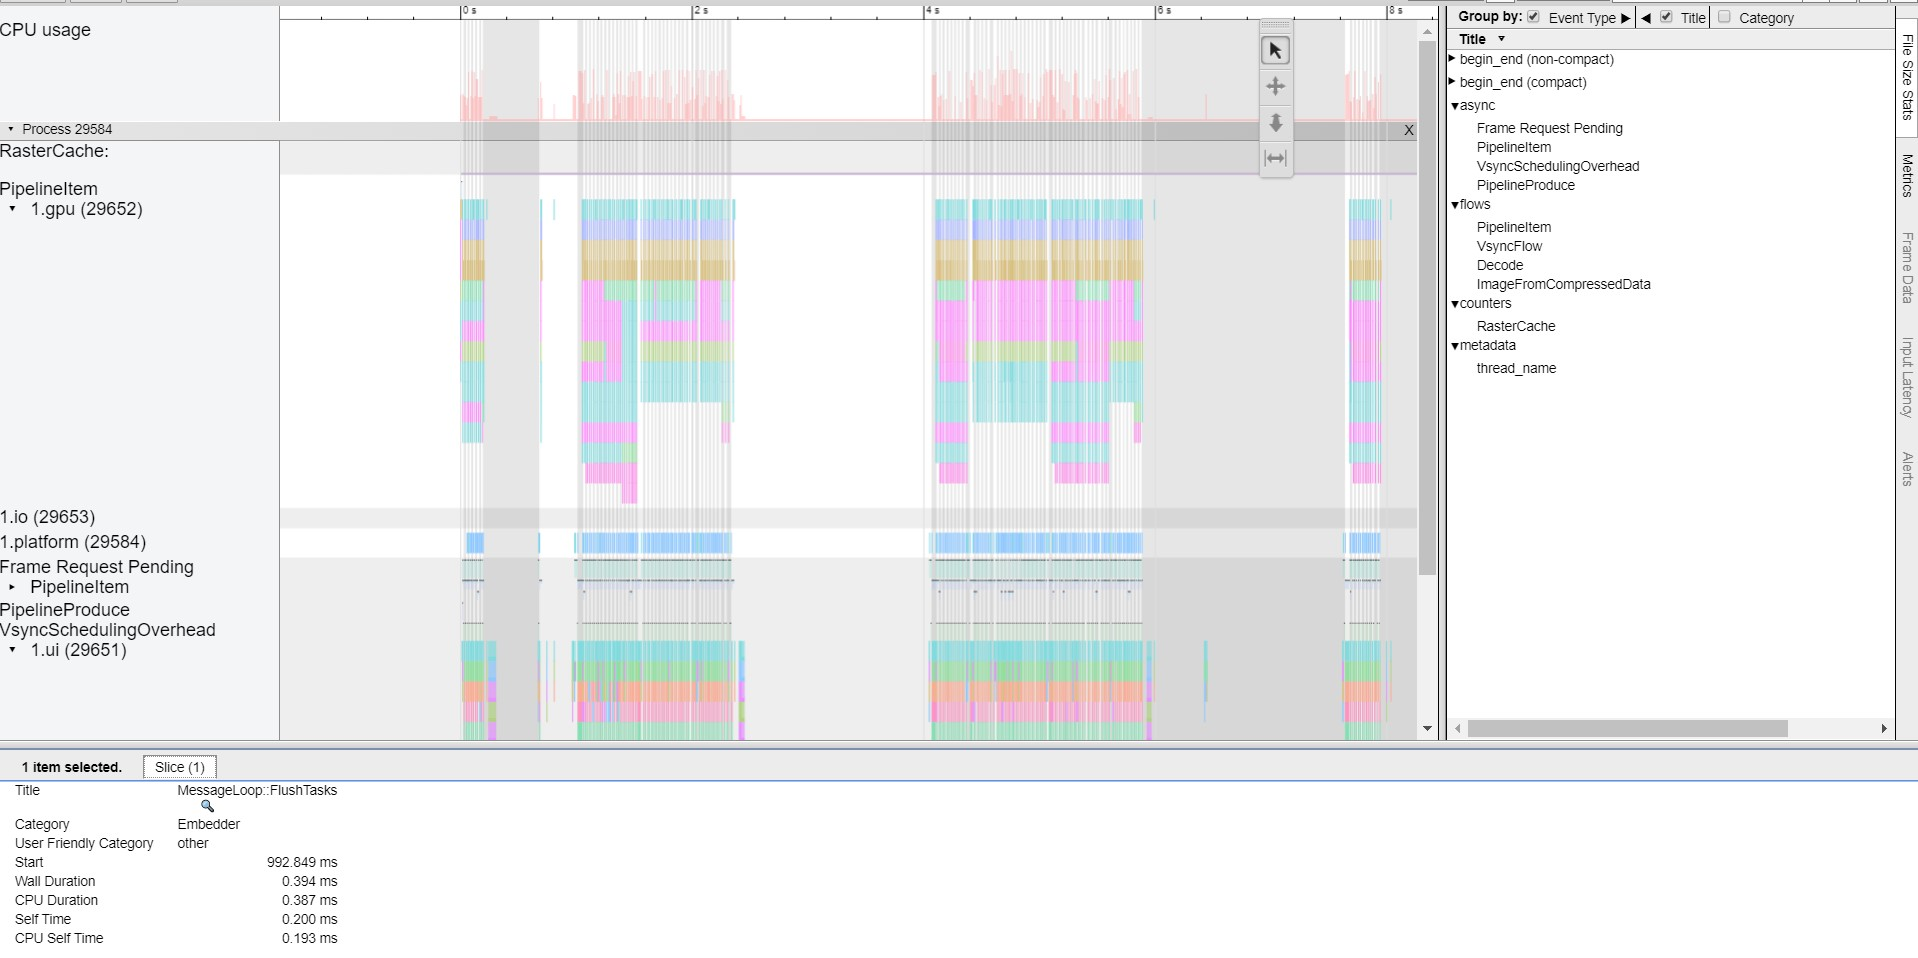
\includegraphics[width=\linewidth]{img/methodologie/chrome-tracing-timeline.jpg}
    \caption{Visuele voorstelling van de ruwe uitvoer in chrome://tracing}
    \label{fig:chrome-tracing-timeline}
\end{figure}


\subsection{Test apparaat}
Hoewel een iOS Simulator en een Android Emulator goed van pas komen tijdens de ontwikkeling van een applicatie wordt voor het meten van de resultaten beroep gedaan op een fysiek apparaat. De meetresultaten die verkregen zouden worden op een emulator zullen verre van een realistische reflectie zijn op de verkregen resultaten op een fysiek apparaat. \autocite{Flutter2019c}

Flutter laat het ook niet toe om de profile modus uit te voeren op een emulator.
Het test apparaat is een OnePlus 3T, zie tabel \ref{table:specifications-test-device} voor de specificaties.
Nadat de broncode voor elke State Management benadering en integratie testen geschreven zijn, kunnen de resulaten verworven worden voor het experiment.

Samengevat worden voor elke bendaring de gegeven stappen doorlopen door middel van de Flutter integration tests. Tijdens deze procedure wordt de verworven data weggeschreven in een JSON-bestand. Dit bestan bevat de nodige CPU-waarden om verder te gaan met de analyse van de resulaten.
% TODO: aanvullen? Ja 

\begin{table}[H]
    \centering
    \begin{tabular}{ll}
        Model & A3003 \\
        Besturingssysteem & Android 9.0 - OxygenOS 9.0.6 \\
        Chipset & Qualcomm MSM8996 Snapdragon 821 (14 nm)  \\
        CPU & Quad-core (2x2.35 GHz Kryo \& 2x1.6 GHz Kryo) \\
        GPU &  Adreno 530 \\
        Geheugen & 6GB RAM \\
        Opslag & 64GB \\ 
        &
    \end{tabular}
    \caption{Specificaties van het test apparaat}
    \label{table:specifications-test-device}
\end{table}

%% TODO: Hoe ben je te werk gegaan? Verdeel je onderzoek in grote fasen, en
%% licht in elke fase toe welke stappen je gevolgd hebt. Verantwoord waarom je
%% op deze manier te werk gegaan bent. Je moet kunnen aantonen dat je de best
%% mogelijke manier toegepast hebt om een antwoord te vinden op de
%% onderzoeksvraag.

